\section{OneOcean Suite}
\label{sec:oneocean_suite}

OneOcean combines a shared ocean dataset, two simulation backends, and a ten-task evaluation protocol.

\subsection{Unified spatiotemporal ocean dataset}
\label{sec:env_product}

The shared NetCDF representation harmonizes GEBCO bathymetry with GOPAF currents and optional tides. It exposes named latitude, longitude, time, and depth coordinates, eastward and northward current components, elevation, and a mask for invalid terrain and NoData cells. The pipeline crops the requested region, retains the returned time and depth levels, aligns variables on one horizontal grid, and records provenance.

The core backend selects a fixed $(t,d)$ slice for deterministic rollouts, whereas the external backend advances a dataset clock. Table~\ref{tab:data_variants} reports the realized products: the 0--200\,m requests returned 26 levels through 186.13\,m, while \texttt{tiny} contains one near-surface level at 0.494\,m. Appendix Sec.~\ref{supp-app:data} specifies the full schema, mask semantics, coordinate conventions, validation results, and tide sampling and depth treatment.

The validity mask marks unusable cells. The tide-enabled \texttt{scene} variant aligns tide samples to the dataset clock and applies depth attenuation.

\begin{table}[!t]
\centering
\scriptsize
\setlength{\tabcolsep}{2.2pt}
\renewcommand{\arraystretch}{1.08}
\begin{tabularx}{\columnwidth}{@{}l>{\raggedright\arraybackslash}p{0.30\columnwidth}>{\centering\arraybackslash}p{0.24\columnwidth}>{\raggedright\arraybackslash}X@{}}
\toprule
\textbf{Variant} & \textbf{Region and period} & \textbf{$T\!\times\!D\!\times\!H\!\times\!W$} & \textbf{Resolution; size; use} \\
\midrule
\texttt{tiny} & 42.1--42.7 N, 71.2--70.2 W; 2025 & $357\!\times\!1\!\times\!62\!\times\!101$ & $\approx0.01^\circ$; 29 MB; tests and web \\
\texttt{scene} & 32--33 N, 66.5--65.5 W; Dec. 2025 & $23\!\times\!26\!\times\!240\!\times\!240$ & $0.00418^\circ$; 690 MB; scenes \\
\texttt{public} & 30--40 N, 72--62 W; 2025 & $357\!\times\!26\!\times\!41\!\times\!41$ & $0.25^\circ$; 175 MB; release \\
\bottomrule
\end{tabularx}
\caption{Realized combined NetCDF variants. Sizes are the merged products themselves; source subsets and derived assets are distributed separately.}
\label{tab:data_variants}
\end{table}

\subsection{Data-grounded disturbance signals}
\label{sec:signals}

OneOcean exports either a fixed gridded slice for high-throughput rollouts or a temporal profile for scene-backed execution. Both apply current through a recorded relative-velocity convention in the core frame $(x,y,z)=$(east, depth-down, north), and every artifact records its extraction indices. Figure~\ref{fig:base_current_field} shows one current slice over bathymetry; Appendix Sec.~\ref{supp-app:data} details sampling, export, and provenance.

\begin{figure}[t]
 \centering
 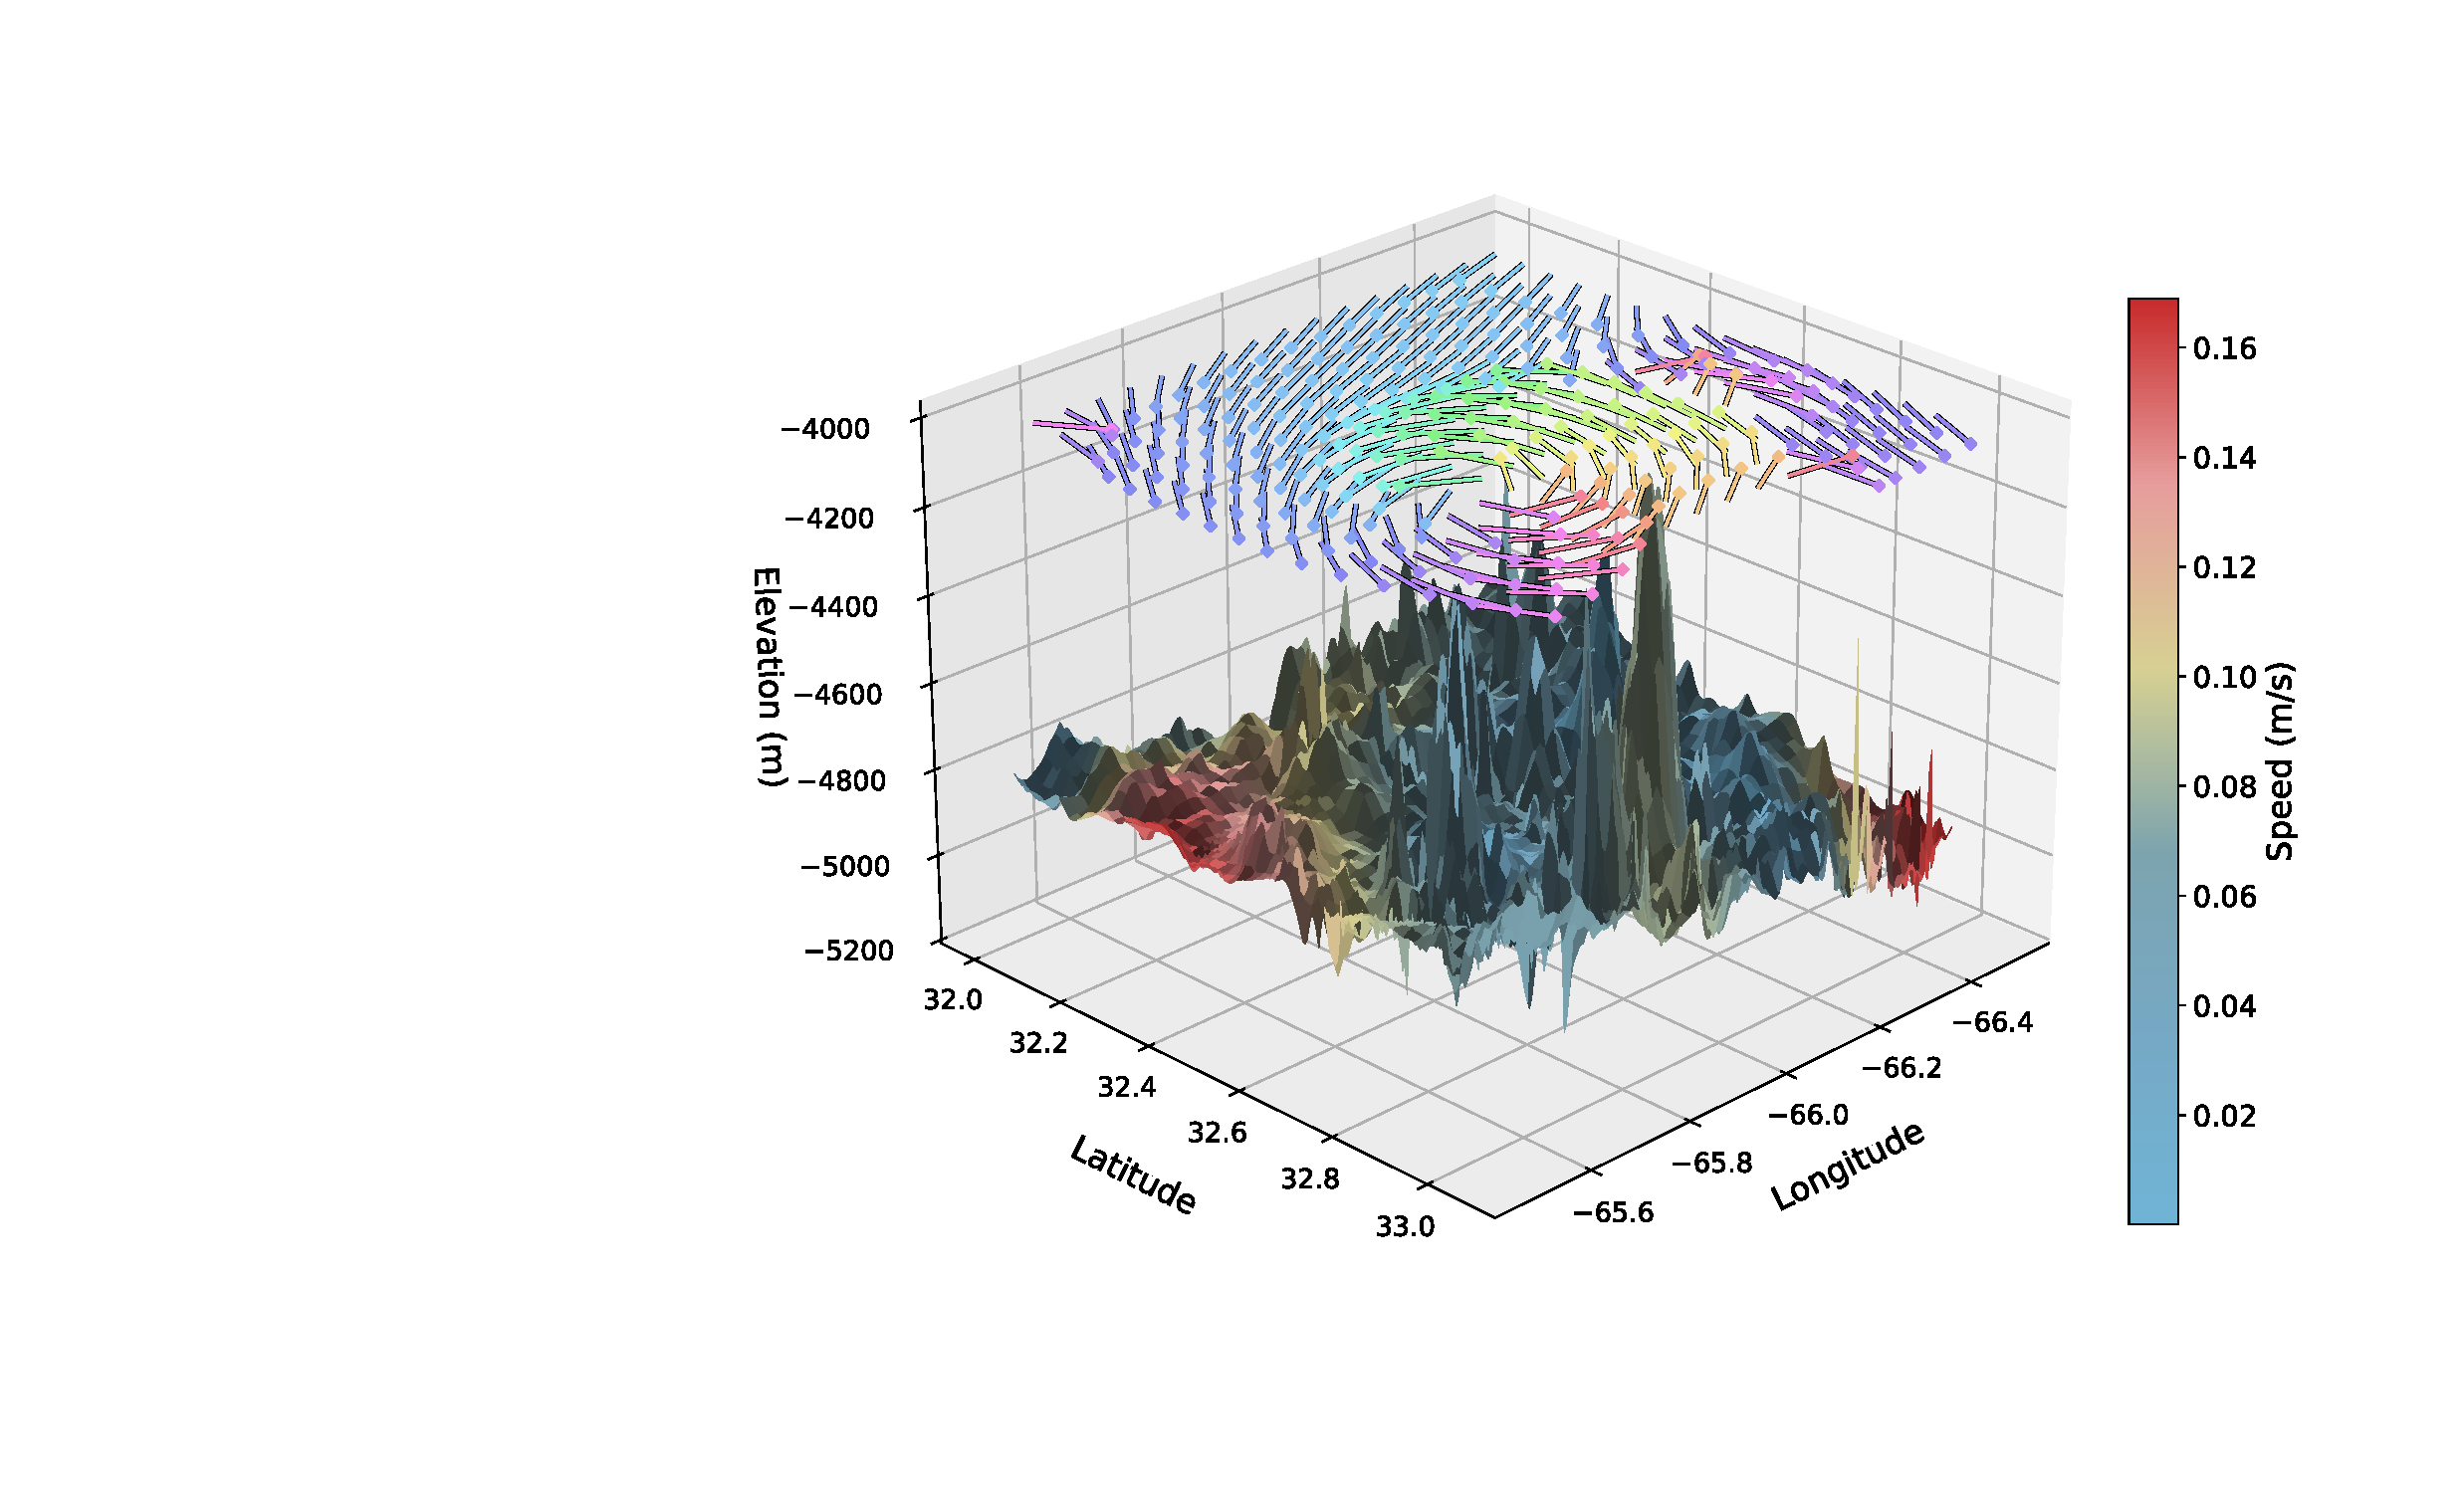
\includegraphics[width=0.98\linewidth]{figures/ocpnet_base_current_3d_diffusion_el25_az045.pdf}
 \caption{Base current field visualization over bathymetry. The horizontal current components are $u_{\mathrm{data}}$ and $v_{\mathrm{data}}$; surface color indicates speed magnitude (m\,s$^{-1}$). View configuration: pitch $25^\circ$, azimuth $45^\circ$, and depth index $0$ (source depth 0.494\,m). The terrain surface is colored by speed and overlaid with arrows indicating current direction.}
 \label{fig:base_current_field}
\end{figure}

\paragraph{Environment queries and probes.}
\label{sec:queries_probes}

Shared queries expose local current, bathymetry, mask validity, and task signals. Pollution tasks observe $o_i^c(t)=C(p_i(t),t)$ from either a current-advected Gaussian or an Ocean Current Prediction Network (OCPNet) field. Both models generate reproducible synthetic concentration signals. Appendix Sec.~\ref{supp-app:models_ros} gives the probe, sink, and discrete-source cleanup semantics.

\subsection{Task suite and difficulty tiers}
\label{sec:tasks}

OneOcean defines ten tasks spanning navigation and tracking (G2G, SK, RF, DPT), sensing and inspection (AS, PI), and coordination and pollution response (FT, SPC, UPL, FH). Table~\ref{tab:task_ladder} gives team sizes and primary metrics; Appendix Sec.~\ref{supp-app:tasks} provides the complete objectives, observations, constraints, and success conditions.

\begin{table}[!t]
\centering
\scriptsize
\setlength{\tabcolsep}{3pt}
\renewcommand{\arraystretch}{1.08}
\begin{tabular*}{\columnwidth}{@{\extracolsep{\fill}}>{\raggedright\arraybackslash}p{0.18\columnwidth}c c c >{\raggedright\arraybackslash}p{0.28\columnwidth}@{}}
\toprule
\textbf{Category} & \textbf{Task} & \textbf{Agents} & \textbf{Goal} & \textbf{Primary metric} \\
\midrule
Navigation & \textbf{G2G} & 1 & reach & final goal error \\
Navigation & \textbf{SK} & 1 & hold & station root-mean-square error \\
Navigation & \textbf{RF} & 1 & follow & cross-track error \\
Navigation & \textbf{DPT} & 1 & track & depth-tracking error \\
\makecell[l]{Sensing and\\Coverage} & \textbf{AS} & 1--10 & scan & coverage fraction \\
\makecell[l]{Sensing and\\Inspection} & \textbf{PI} & 1--10 & inspect & inspection score \\
Coordination & \textbf{FT} & 2--10 & transit & formation error \\
Pollution & \textbf{SPC} & 2--10 & clean & cleanup rate \\
Coordination & \textbf{UPL} & 5 & lift & lift success \\
Coordination & \textbf{FH} & 8 & herd & containment success \\
\bottomrule
\end{tabular*}
\caption{The OneOcean task suite (10 tasks). Each task is evaluated at Tiers 1--3 and paired with a compact goal type and a primary task-specific metric.}
\label{tab:task_ladder}
\end{table}

\revise{Tiers 1, 2, and 3 jointly increase current strength, precision, route and coverage extent, sensing difficulty, and coordination tightness while preserving each task's interface. Every task declares its objective, observations, feasibility constraints, success condition, and primary metric. The release also includes a lightweight Robot Operating System 2 (ROS~2) bridge for state, probes, and velocity commands; its frames, topics, services, and interface checks appear in Appendix Sec.~\ref{supp-app:models_ros}.}

Navigation and tracking tasks test disturbance rejection and sustained trajectory accuracy; sensing and inspection tasks require spatial coverage or physical cue encounters; coordination and pollution tasks add team geometry, assignment, and dwell-time coupling. We report success together with task-specific progress.

\revise{
\begin{table*}[!t]
\centering
\scriptsize
\setlength{\tabcolsep}{1.2pt}
\renewcommand{\arraystretch}{1.10}
\begin{tabularx}{\textwidth}{@{}l*{3}{Y}|*{3}{Y}|*{6}{Y}@{}}
\toprule
\multirow{2}{*}{\textbf{Method}} & \multicolumn{3}{c}{\textbf{Macro (Tier 2)}} & \multicolumn{3}{c}{\textbf{Macro (Tier 3)}} & \multicolumn{6}{c}{\textbf{Tier 3 key-task metrics}} \\
\cmidrule(lr){2-4}\cmidrule(lr){5-7}\cmidrule(lr){8-13}
 & \makecell{Suite\\SR(\%)} & \textbf{$E$} & \makecell{Coll.\\(\%)} & \makecell{Suite\\SR(\%)} & \textbf{$E$} & \makecell{Coll.\\(\%)} & \makecell{G2G\\SR(\%)} & \makecell{RF\\SR(\%)} & \makecell{SK\\RMS} & \makecell{Scan\\cov.} & \makecell{Pipe\\score} & \makecell{Cleanup\\rate} \\
\midrule
\rowcolor{oursbg}
Heuristic & \best{84.6} & 1842.3 & \best{5.68} & \best{29.0} & 3352.4 & 8.19 & \best{74.0} & \best{54.0} & \best{1.07} & \best{0.89} & \best{0.78} & \best{0.56} \\
BC & 58.6 & \best{1271.2} & 9.72 & 6.0 & \best{1635.1} & \best{6.41} & 34.0 & 0.0 & 26.52 & 0.89 & 0.67 & 0.06 \\
\bottomrule
\end{tabularx}
\caption{Headline core-benchmark results (6DoF): macro averages at Tiers 2 and 3 plus Tier 3 key-task metrics, using 50 episodes per task and tier. Success Rate (SR) is reported in percent; Macro Suite SR is an unweighted mean across the 10 tasks. Coll is the mean collision-step ratio (\%) with a 2.0\,m radius. Best values per column are highlighted.}
\label{tab:headline_macro_keymetrics}
\end{table*}
}

\revise{
\begin{table*}[t]
\centering
\scriptsize
\setlength{\tabcolsep}{1.5pt}
\renewcommand{\arraystretch}{1.10}
\begin{tabularx}{\textwidth}{@{}l*{9}{Y}@{}}
\toprule
\textbf{Method} & \makecell{Avg.\\SR(\%)} & \makecell{Cleanup\\SR(\%)} & \makecell{Cleanup\\rate} & \makecell{Scan\\SR(\%)} & \makecell{Scan\\cov.} & \makecell{Pipe\\SR(\%)} & \makecell{Pipe\\score} & \textbf{$T$(s)} & \textbf{$E$} \\
\midrule
\rowcolor{oursbg}
Heuristic & \best{65.8} & 60.0 & \best{0.87} & \best{77.5} & 0.80 & \best{60.0} & \best{0.69} & \best{776.8} & 9132.4 \\
BC & 45.0 & 10.0 & 0.32 & 67.5 & 0.79 & 57.5 & 0.61 & 921.6 & \best{6908.2} \\
LLM-ChatGLM3-6B & 55.0 & 60.0 & \best{0.87} & 77.5 & \best{0.82} & 27.5 & 0.54 & 860.3 & 9671.5 \\
LLM-Qwen2.5-7B & 47.5 & 57.5 & 0.81 & 57.5 & 0.78 & 27.5 & 0.57 & 1077.2 & 11703.8 \\
LLM-Qwen2-7B & 45.0 & 57.5 & 0.86 & 67.5 & 0.81 & 10.0 & 0.51 & 991.4 & 10422.1 \\
LLM-Mistral-7B & 42.5 & 55.0 & 0.82 & 55.0 & 0.78 & 17.5 & 0.52 & 1044.2 & 11288.9 \\
LLM-Llama3-8B & 44.2 & \best{67.5} & 0.84 & 47.5 & 0.77 & 17.5 & 0.59 & 1099.1 & 11614.2 \\
LLM-Llama2-7B & 30.8 & 55.0 & \best{0.87} & 27.5 & 0.75 & 10.0 & 0.46 & 1156.4 & 11654.3 \\
\bottomrule
\end{tabularx}
\caption{Core-benchmark planning-suite performance at Tier 2 with doubled currents: heuristic vs BC vs local LLM planners on three planning-sensitive tasks, using 40 episodes per task (120 per method). Best values per column are highlighted.}
\label{tab:planning_suite_perf_t2}
\end{table*}
}


\subsection{Two execution backends}
\label{sec:backends}

The two backends share task definitions and reporting formats. The headless \textbf{core benchmark backend} consumes a NumPy Archive (NPZ) current slice and task and action configurations. It returns observations, metrics, run records, and recorder streams, and supports 3--6 DoF vehicle dynamics (6DoF in the main experiments) \cite{UUVSim}. The \textbf{external underwater-scene backend} runs the task suite in packaged underwater scenes using a temporal OneOcean current export. It returns route and task metrics alongside simulation recordings.

\paragraph{Benchmark protocol and metrics.}
\label{sec:protocol}

\begin{figure}[!b]
 \centering
 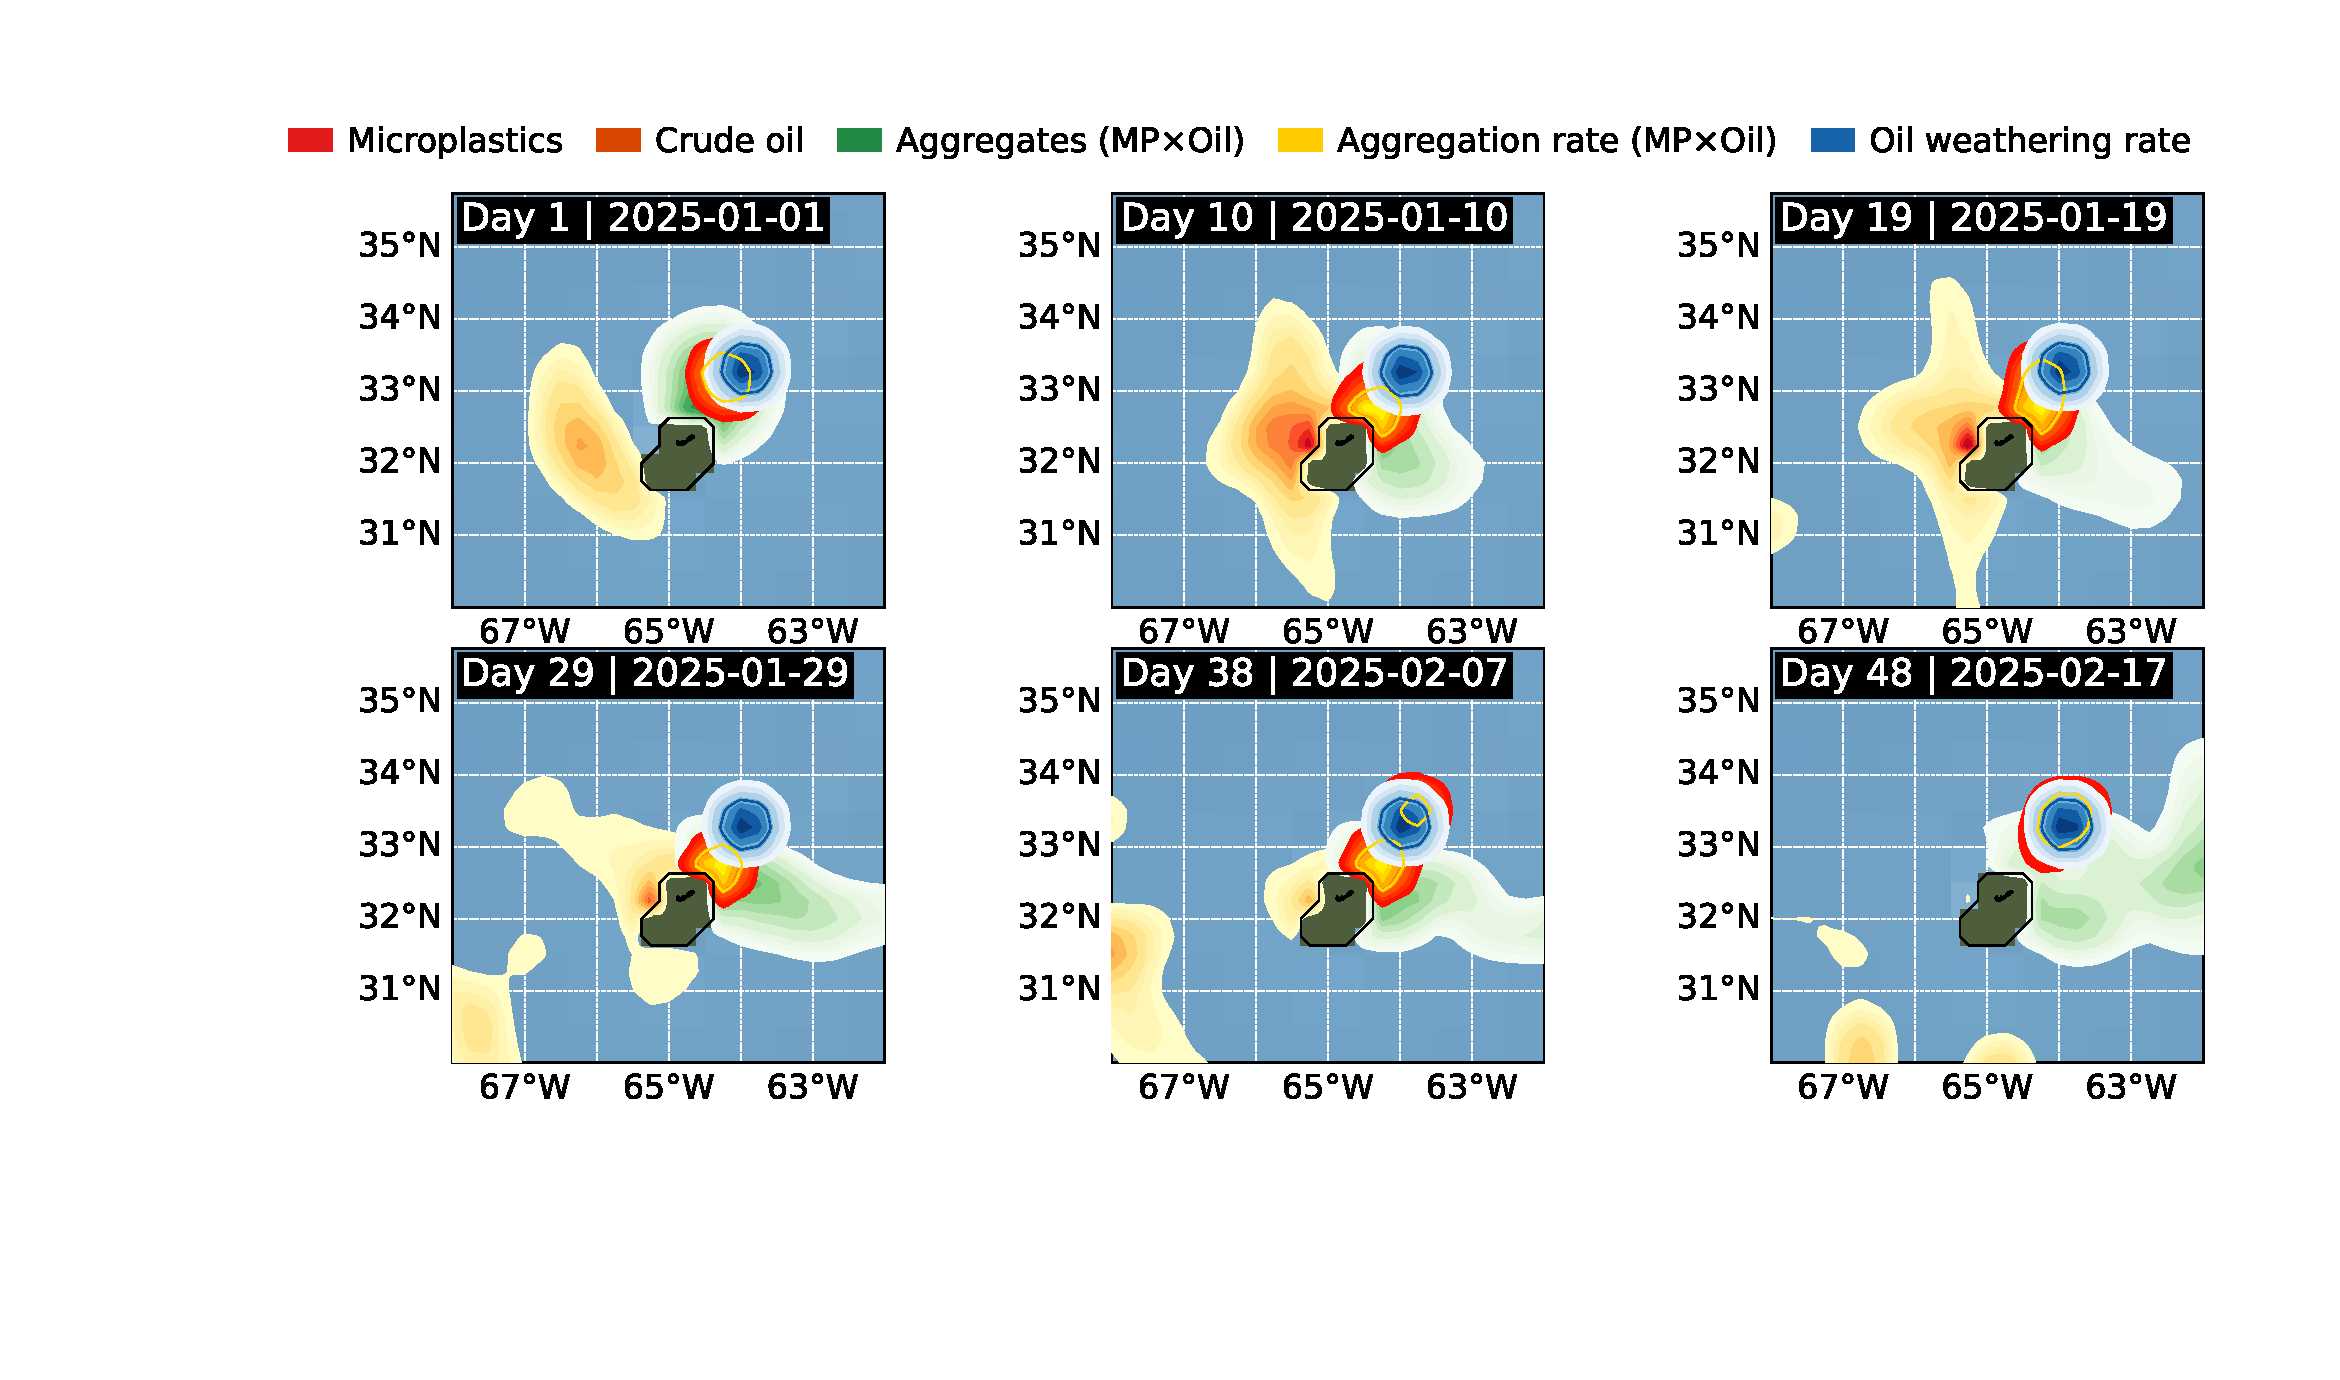
\includegraphics[width=0.98\linewidth]{figures/ocpnet_multispecies_seed04_panel.pdf}
 \caption{OCPNet multispecies diffusion and reaction fields that can generate concentration observations for localization, containment, and cleanup tasks.}
 \label{fig:ocpnet_panels}
\end{figure}

\revise{Actions specify desired relative velocity, clipped as $a_t=\mathrm{clip}(\tilde a_t;v_{\max})$. With current gain $g$,}
\begin{equation}
\revise{c_t = g\,[u_{\mathrm{data}}(x_t,z_t),\,0,\,v_{\mathrm{data}}(x_t,z_t)] + c_{\mathrm{tide}}(t),}
\end{equation}
\revise{where $u_{\mathrm{data}}$ and $v_{\mathrm{data}}$ are sampled horizontal currents and $c_{\mathrm{tide}}$ is an optional synthetic robustness signal. With body velocity $\nu=[\nu_\ell^\top,\nu_a^\top]^\top$, rotation $R$, and diagonal $M,D,K_\ell,K_a,K_d$, the diagonal 6DoF update is}
\begin{align}
M\dot\nu &= \tau-D\nu, &
\tau_\ell &= K_\ell(\nu_\ell^{\rm cmd}-\nu_\ell), \nonumber\\
\tau_a &= K_a(\nu_a^{\rm cmd}-\nu_a)-K_d\nu_a, &
\dot p &= R\nu_\ell+c_t .
\end{align}
\revise{Commands are transformed to the body frame; yaw follows horizontal motion while roll and pitch are stabilized. Kinematic mode directly integrates $a_t+c_t$, and 3DoF suppresses roll and pitch. The model uses diagonal inertia and damping, bounded attitude, and externally sampled current transport. Added mass, Coriolis and restoring terms, thruster allocation, and two-way fluid coupling are omitted. Hard terrain feasibility is}
\begin{equation}
\mathcal C=\{(x,y,z)\mid m_{\mathrm{land}}(x,z)<\tau_{\mathrm{land}},\ y+\delta_{\mathrm{clr}}\le-h(x,z)\},
\end{equation}
\revise{where $m_{\mathrm{land}}$ is mask validity, $h$ is bathymetric elevation, and $\delta_{\mathrm{clr}}$ is required clearance. Masked, out-of-bounds, or clearance-violating proposals are rejected through the shared constraint path. We report SR, timeout-aware episode time $T$, $E=\sum_t\|a_t\|_2^2\Delta t$, near-collision ratio, and task-specific metrics.}

\revise{BC maps normalized goal, depth, probe, current, and task features $\phi_t$ to $\hat a_t=f_\theta(\phi_t)$ and minimizes the heuristic-action loss}
\begin{equation}
\mathcal L_{\mathrm{BC}}=N_{\mathrm{BC}}^{-1}\sum_t\|a_t^{\mathrm{heur}}-\hat a_t\|_2^2.
\end{equation}
\revise{Every $K$ steps, an LLM instead proposes a discrete assignment $g_k=\pi_{\mathrm{LLM}}(s_k)$; schema-invalid output invokes a deterministic allocator, and a shared low-level controller executes $a_t=\pi_{\mathrm{low}}(x_t,g_k)$. Appendix Sec.~\ref{supp-app:models_ros} gives dynamics defaults, pollution semantics, and ROS mapping; Appendix Sec.~\ref{supp-app:protocol} defines all metrics and manifests.}

\paragraph{Optional pollution fields (OCPNet).}
\label{sec:ocpnet}

\revise{Continuous containment applies a local concentration sink. SPC completes discrete sources after an assignment-and-dwell condition; its cleanup rate is the fraction of sources completed. Figure~\ref{fig:ocpnet_panels} shows the multispecies concentration signal.}
